\documentclass[a4paper,11pt]{article}
\usepackage{filecontents}

\usepackage[utf8]{inputenc}
\usepackage[english]{babel}
\usepackage{graphicx, array, blindtext}
\usepackage[colorinlistoftodos]{todonotes}
\DeclareUnicodeCharacter{2212}{-}
\usepackage [a4 paper , hmargin = 1.2 in , bottom = 1.5 in] {geometry}
\usepackage [parfill] {parskip}

\usepackage{enumitem}
\usepackage{amsmath}
\usepackage{amsthm}

\usepackage{nameref}
\usepackage{amssymb}
\usepackage [linesnumbered, ruled, vlined] {algorithm2e}
\usepackage{listings}
\usepackage{xcolor}
\usepackage{floatrow}
\usepackage{siunitx}
\usepackage{cancel}
\usepackage{fancyhdr}
\usepackage{graphicx}
\usepackage{verbatim}
\usepackage[document]{ragged2e}

\renewcommand{\footrulewidth}{0.4pt}
\newtheorem{definition}{Definition}
\numberwithin{definition}{section}
\newtheorem{mytheorem}{Theorem}
\numberwithin{mytheorem}{subsection}
\newcommand{\notimplies}{\;\not\!\!\!\longrightarrow}  
\newcommand\norm[1]{\left\lVert#1\right\rVert}
\pagestyle{fancy}
\fancyhf{}
\rhead{CS754 Assignment 3}
\lhead{200050013-200050130}
\fancyfoot[C]{Page \thepage}
\usepackage{subcaption}
\usepackage{listings}


\usepackage{hyperref}
\urlstyle{same}
\hypersetup{pdftitle={main.pdf},
    colorlinks=false,
    linkbordercolor=red
}
\usepackage{array}
\usepackage{listings,chngcntr}

\begin{document}
\centering{

\title{\fontsize{150}{60}{CS754 Assignment 3 Report}}

\author{
Arpon Basu \\ Shashwat Garg }
}

\date{Spring 2022}
\maketitle

\justifying
\tableofcontents

\newpage
\justifying
\section*{Introduction}

Welcome  to our report on CS754 Assignment 3. We have tried to make this report comprehensive and self-contained. We hope reading this would give you a proper flowing description of our work, methods used and the results obtained.

Also note that we installed the \texttt{Image Processing Toolbox} in MATLAB for this assignment. Thus the grader is urged to install it if she wishes to run the code on her on her machine.

Hope you enjoy reading the report. Here we go!


\section{Problem 1}
For this problem we implemented the ISTA algorithm as was mentioned in the lecture slides and used it for both parts. For further perusal, we encourage the grader to check the code files submitted.\\
(a) In this part, we read the image, vectorized it, and added some noise to it (since noise of variance 3 was required, we took a Gaussian Random Variable vector with variance 1 and multiplied it by $\sqrt{3}$ to make the variance 3). Since natural images are assumed to be sparse in orthonormal bases like the 2D-DCT, the matrix for our ISTA cost function was the DCT matrix itself. \\
Thus our cost function was
$$J(\theta) = \lVert y - U\theta\rVert^2_2 + \lambda\lVert\theta\rVert_1$$
where $y$ is the vectorized noisy image.\\
In our code, we took $\lambda = 1$, and we also took $\alpha = 1$ (note that since $U$ is orthonormal, the largest eigenvalue of $U^*U$ is 1 itself).\\
Also, since the basis matrix for the 256$\times$256 images was too large to store in memory, we performed our computations patch-wise, in overlapping patches of 8$\times$8 and a stride of 1.\\
We got a RMSE error of 13.81\% after all the overlapping images were summed up and averaged accordingly.
Attached below is the reconstructed image for the graders perusal:
\begin{figure}[H]
    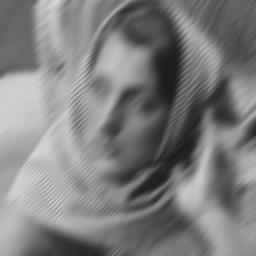
\includegraphics{1a.jpg}
    \caption{Reconstructed image for the first part}
\end{figure}
(b) For the second part, we reused the same ISTA and other utility function codes from the first part. However, here the matrix was slightly different, ie:- 
$$J(\theta) = \lVert y - \Phi U\theta\rVert^2_2 + \lambda\lVert\theta\rVert_1$$
, and thus $A = \Phi U$, where $\Phi\in\mathbb{R}^{32\times 64}$ is a matrix of i.i.d unit Gaussian RVs. \\
The hyperparameter $\lambda$ was kept 1 here too. However, this time $\alpha$ in the ISTA algorithm had to be chosen to be the largest eigenvalue of $A^*A$. We also added a 1 to that to avoid numerical stability issues.\\
% Keeping the remaining factors same as in the previous part (same 8$\times$8 patches, stride to be 1),we got a reconstruction error of 
PART B REMAINS TO BE DONE. ERROR SUDDENLY BLEW UP TO 50 \%.  
\section{Problem 2}
% (a) The restricted eigenvalue property has a very neat and succinct description in terms of the SVD of our sensing matrix $\boldsymbol{X}$, and that's how we'll define it.\\
% Note that the restricted eigenvalue property for the matrix $X$ is defined as follows
% $$\frac{1}{N\cdot \lVert\nu\rVert_2^2}\nu^TX^TX\nu \geq \gamma \;\forall\;\nu \in \mathbb{K}^{p\times 1}\setminus\{\mathbf{0}\}$$
% where $\gamma$ is the coefficient of the property.\\
% Now, notice that if we restrict $\nu$ to vary over only unit length vectors in $\mathbb{K}^{p\times 1}$, then we can get rid of the $\lVert\nu\rVert_2^2$ in the denominator. Also, since the inequality holds for all $\nu$ in our chosen space, it's enough to assume that the infimum of the expression $\frac{1}{N}\nu^TX^TX\nu$ over all $\nu$ such that $\lVert\nu\rVert_2 = 1$ must be greater than or equal to $\gamma$, ie:- 
% $$\mathrm{min}_{\lVert\nu\rVert_2 = 1}\frac{1}{N}\nu^TX^TX\nu \geq \gamma$$
% $$\implies \mathrm{min}_{\lVert\nu\rVert_2 = 1}(X\nu)^TX\nu \geq N\gamma$$
% $$\implies \mathrm{min}_{\lVert\nu\rVert_2 = 1}\lVert X\nu\rVert_2^2 \geq N\gamma$$
% $$\implies \mathrm{min}_{\lVert\nu\rVert_2 = 1}\lVert X\nu\rVert_2 \geq \sqrt{N\gamma}$$
% But from the theory of Singular Value Decomposition, we know that $\mathrm{min}_{\lVert\nu\rVert_2 = 1}\lVert X\nu\rVert_2$ is equal to the smallest singular value of $X$.\\
% Thus, we can \textbf{define} the \textbf{Restricted Eigenvalue Property} with coefficient $\gamma$ as follows : The matrix $\boldsymbol{X}\in\mathbb{R}^{n\times p}$ is said to satisfy the Restricted Eigenvalue Property with coefficient $\gamma$ if the \textbf{smallest singular value of $\boldsymbol{X}$ is atleast $\sqrt{N\gamma}$}.\\
(a) The restricted eigenvalue condition is defined as follows:\\
The matrix $\boldsymbol{X}\in\mathbb{R}^{n\times p}$ is said to satisfy the Restricted Eigenvalue Property over a constraint set $\mathcal{C}$ with coefficient $\gamma$ if 
$$\frac{1}{N\cdot \lVert\nu\rVert_2^2}\nu^TX^TX\nu \geq \gamma \;\forall\;\nu \in \mathcal{C}\setminus\{\mathbf{0}\}$$
$$\implies \frac{1}{N\cdot \lVert\nu\rVert_2^2}(X\nu)^TX\nu \geq \gamma\;\forall\;\nu \in \mathcal{C}\setminus\{\mathbf{0}\}$$
$$\implies \frac{1}{N}\lVert X\nu\rVert^2_2 \geq \gamma\lVert\nu\rVert_2^2\;\forall\;\nu \in \mathcal{C}$$
Thus our definition condenses to:
\textbf{The matrix $\boldsymbol{X}\in\mathbb{R}^{n\times p}$ is said to satisfy the Restricted Eigenvalue Property over a constraint set $\mathcal{C}$ with coefficient $\gamma$ if }
$$\boldsymbol{\frac{1}{N}\lVert X\nu\rVert^2_2 \geq \gamma\lVert\nu\rVert_2^2\;\;\forall\nu\in\mathcal{C}}$$
(b) We have that 
$$G(\nu) := \frac{1}{2N}\lVert y - X(\beta^{*} + \nu)\rVert^2_2 + \lambda_N\lVert\beta^{*} + \nu\rVert_1$$
$$J(\boldsymbol{x}) := \frac{1}{2N}\lVert y - X\boldsymbol{x}\rVert^2_2 + \lambda_N\lVert\boldsymbol{x}\rVert_1$$
Thus 
$$G(0) := \frac{1}{2N}\lVert y - X\beta^{*}\rVert^2_2 + \lambda_N\lVert\beta^{*}\rVert_1 = J(\beta^{*})$$
On the other hand, for $\widehat{\nu} := \widehat{\beta} - \beta^{*}$, we have
$$G(\widehat{\nu}) := \frac{1}{2N}\lVert y - X\widehat{\beta}\rVert^2_2 + \lambda_N\lVert\widehat{\beta}\rVert_1 = J(\widehat{\beta})$$
But $\widehat{\beta}$ was, \textbf{by construction} (as mentioned on Pg\# 308, third last line), the optimizer of the LASSO function $J(\boldsymbol{x})$, and consequently $G(\widehat{\nu}) = J(\widehat{\beta}) \leq J(\beta^*) = G(0)$, as desired.\\
(c) We just have to piece together some equations and inequalities to derive equation 11.21. They go as follows:
$$G(\widehat{\nu}) \leq G(0)$$
$$y = X\beta^* + w$$
$$\widehat{\beta} = \beta^* + \widehat{\nu}$$
The first inequality $G(\widehat{\nu}) \leq G(0)$, combined with the fact that $\widehat{\beta} = \beta^* + \widehat{\nu}$ yields
$$G(\widehat{\nu}) \leq G(0)$$
$$\implies \frac{1}{2N}\lVert y - X\widehat{\beta}\rVert^2_2 + \lambda_N\lVert\widehat{\beta}\rVert_1 \leq \frac{1}{2N}\lVert y - X\beta^{*}\rVert^2_2 + \lambda_N\lVert\beta^{*}\rVert_1$$
$$\implies \frac{1}{2N}\lVert y - X(\beta^* + \widehat{\nu})\rVert^2_2 + \lambda_N\lVert\beta^* + \widehat{\nu}\rVert_1 \leq \frac{1}{2N}\lVert y - X\beta^{*}\rVert^2_2 + \lambda_N\lVert\beta^{*}\rVert_1$$
Now, using the fact that $y = X\beta^* + w$, we get
$$\frac{1}{2N}\lVert y - X(\beta^* + \widehat{\nu})\rVert^2_2 + \lambda_N\lVert\beta^* + \widehat{\nu}\rVert_1 \leq \frac{1}{2N}\lVert y - X\beta^{*}\rVert^2_2 + \lambda_N\lVert\beta^{*}\rVert_1$$
$$\implies \frac{1}{2N}\lVert y - X\beta^* - X\widehat{\nu}\rVert^2_2 + \lambda_N\lVert\beta^* + \widehat{\nu}\rVert_1 \leq \frac{1}{2N}\lVert w\rVert^2_2 + \lambda_N\lVert\beta^{*}\rVert_1$$
$$\implies \frac{1}{2N}\lVert w - X\widehat{\nu}\rVert^2_2 \leq \frac{1}{2N}\lVert w\rVert^2_2 + \lambda_N(\lVert\beta^{*}\rVert_1 - \lVert\beta^* + \widehat{\nu}\rVert_1)$$
Now, $\lVert w - X\widehat{\nu}\rVert^2_2 = (w - X\widehat{\nu})^T\cdot(w - X\widehat{\nu}) = \lVert w\rVert^2_2 + \lVert X\widehat{\nu}\rVert^2_2 - 2w^TX\widehat{\nu} $. Substituting this in the equation above yields
$$\frac{1}{2N}(\lVert w\rVert^2_2 + \lVert X\widehat{\nu}\rVert^2_2 - 2w^TX\widehat{\nu}) \leq \frac{1}{2N}\lVert w\rVert^2_2 + \lambda_N\{\lVert\beta^{*}\rVert_1 - \lVert\beta^* + \widehat{\nu}\rVert_1\}$$
$$\implies \frac{1}{2N}(\lVert X\widehat{\nu}\rVert^2_2 - 2w^TX\widehat{\nu}) \leq \lambda_N\{\lVert\beta^{*}\rVert_1 - \lVert\beta^* + \widehat{\nu}\rVert_1\}$$
$$\implies \frac{1}{2N}\lVert X\widehat{\nu}\rVert^2_2 - \frac{1}{N}w^TX\widehat{\nu}\leq \lambda_N\{\lVert\beta^{*}\rVert_1 - \lVert\beta^* + \widehat{\nu}\rVert_1\}$$
$$\implies \frac{\lVert X\widehat{\nu}\rVert^2_2}{2N} \leq \frac{w^TX\widehat{\nu}}{N} + \lambda_N\{\lVert\beta^{*}\rVert_1 - \lVert\beta^* + \widehat{\nu}\rVert_1\}$$
as desired.\\
(d) We use a version of H\"{o}lder's inequality for vectors as follows:\\
Let $p, q\in[1,\infty]$ be two real numbers such that $\frac{1}{p} + \frac{1}{q} = 1$. Let $\boldsymbol{x} = (x_1, x_2, ..., x_n)$ and $\boldsymbol{y} = (y_1, y_2, ..., y_n)$ be two vectors. Then
$$\boldsymbol{\sum^{n}_{k = 1}|x_ky_k|\leq (\sum^{n}_{k = 1}|x_k|^p)^{\frac{1}{p}}(\sum^{n}_{k = 1}|y_k|^q)^{\frac{1}{q}} = \lVert x\rVert_p\lVert y\rVert_q}$$
We augment this inequality for our purposes: Note that $\boldsymbol{x}\cdot\boldsymbol{y} = \sum^{n}_{k = 1}x_ky_k \leq \sum^{n}_{k = 1}|x_ky_k| \leq (\sum^{n}_{k = 1}|x_k|^p)^{\frac{1}{p}}(\sum^{n}_{k = 1}|y_k|^q)^{\frac{1}{q}}$, thus showing that $\boldsymbol{x}\cdot\boldsymbol{y}\leq (\sum^{n}_{k = 1}|x_k|^p)^{\frac{1}{p}}(\sum^{n}_{k = 1}|y_k|^q)^{\frac{1}{q}} = \lVert \boldsymbol{x}\rVert_p\lVert \boldsymbol{y}\rVert_q$.\\
In our context let $\boldsymbol{x} = X^Tw$ and $\boldsymbol{y} = \nu$, and let $p =\infty$, $q = 1$. Then, $(X^Tw)\cdot\nu = (X^Tw)^T\nu = w^TX\nu$. Then we have that 
$$(X^Tw)\cdot\nu\leq \lVert X^Tw\rVert_{\infty}\lVert \nu\rVert_1$$
$$\implies w^TX\nu\leq \lVert X^Tw\rVert_{\infty}\lVert \nu\rVert_1$$
Thus, 
$$\frac{w^TX\widehat{\nu}}{N} + \lambda_N\{\lVert\widehat{\nu_S}\rVert_1 - \lVert\widehat{\nu_{S^c}}\rVert_1\}\leq \frac{\lVert X^Tw\rVert_{\infty}}{N}\lVert \nu\rVert_1 + \lambda_N\{\lVert\widehat{\nu_S}\rVert_1 - \lVert\widehat{\nu_{S^c}}\rVert_1\}$$
as desired.\\
(e) Let $S$ be the set of indices where $\beta^*$ is non-zero, and let $S^c := [n]\setminus S$. Now, we've already shown that
$$\frac{\lVert X\widehat{\nu}\rVert^2_2}{2N} \leq \frac{w^TX\widehat{\nu}}{N} + \lambda_N\{\lVert\beta^{*}\rVert_1 - \lVert\beta^* + \widehat{\nu}\rVert_1\}$$
Now, 
$$\lVert \beta^* + \widehat{\nu}\rVert_1 = \lVert \beta_S^* + \widehat{\nu_S}\rVert_1 + \lVert \beta_{S^c}^* + \widehat{\nu_{S^c}}\rVert_1 = \lVert \beta_S^* + \widehat{\nu_S}\rVert_1 + \lVert \widehat{\nu_{S^c}}\rVert_1$$
$$\geq \lVert \beta_S^*\rVert_1 -\lVert \widehat{\nu_S}\rVert_1 + \lVert \widehat{\nu_{S^c}}\rVert_1 =  \lVert \beta^*\rVert_1 -\lVert \widehat{\nu_S}\rVert_1 + \lVert \widehat{\nu_{S^c}}\rVert_1$$
$$\implies \lVert\beta^{*}\rVert_1 - \lVert\beta^* + \widehat{\nu}\rVert_1 \geq \lVert \widehat{\nu_S}\rVert_1 - \lVert \widehat{\nu_{S^c}}\rVert_1$$
since $\beta_{S^c}^* = \mathbf{0}$, and applying the triangle inequality.\\
From the previous part, we also know that 
$$\frac{w^TX\widehat{\nu}}{N} + \lambda_N\{\lVert\widehat{\nu_S}\rVert_1 - \lVert\widehat{\nu_{S^c}}\rVert_1\}\leq \frac{\lVert X^Tw\rVert_{\infty}}{N}\lVert \nu\rVert_1 + \lambda_N\{\lVert\widehat{\nu_S}\rVert_1 - \lVert\widehat{\nu_{S^c}}\rVert_1\}$$
$$\implies\frac{w^TX\widehat{\nu}}{N} + \lambda_N\{\lVert\widehat{\nu_S}\rVert_1 - \lVert\widehat{\nu_{S^c}}\rVert_1\}\leq \frac{\lambda_N}{2}\lVert \nu\rVert_1 + \lambda_N\{\lVert\widehat{\nu_S}\rVert_1 - \lVert\widehat{\nu_{S^c}}\rVert_1\}$$
since $\lambda_N \geq 2\frac{\lVert X^Tw\rVert_{\infty}}{N}$ by the premise of the theorem. Finally, note that by the additivity of the $l_1$-norm, 
$$\lVert\widehat{\nu}\rVert_1 = \lVert\widehat{\nu_S}\rVert_1 + \lVert\widehat{\nu_{S^c}}\rVert_1$$
yielding
$$\frac{w^TX\widehat{\nu}}{N} + \lambda_N\{\lVert\widehat{\nu_S}\rVert_1 - \lVert\widehat{\nu_{S^c}}\rVert_1\}\leq \frac{\lambda_N}{2}\{\lVert\widehat{\nu_S}\rVert_1 + \lVert\widehat{\nu_{S^c}}\rVert_1\} + \lambda_N\{\lVert\widehat{\nu_S}\rVert_1 - \lVert\widehat{\nu_{S^c}}\rVert_1\}$$
$$ = \frac{3\lambda_N}{2}\lVert\widehat{\nu_S}\rVert_1 - \frac{\lambda_N}{2}\lVert\widehat{\nu_{S^c}}\rVert_1 \leq \frac{3\lambda_N}{2}\lVert\widehat{\nu_S}\rVert_1$$
For the final step, let $|S| = k$. Then by the RMS-AM inequality on vectors,
$$\frac{\lVert\boldsymbol{x}\rVert_1}{n}\leq\frac{\lVert\boldsymbol{x}\rVert_2}{\sqrt{n}}$$
where $\boldsymbol{x}\in\mathbb{R}^n$.\\
Thus $\lVert\widehat{\nu_S}\rVert_1 \leq \sqrt{|S|}\lVert\widehat{\nu_S}\rVert_2 \leq \sqrt{|S|}\lVert\widehat{\nu}\rVert_2 = \sqrt{k}\lVert\widehat{\nu}\rVert_2$. Combining this with the inequality above yields
$$\frac{w^TX\widehat{\nu}}{N} + \lambda_N\{\lVert\widehat{\nu_S}\rVert_1 - \lVert\widehat{\nu_{S^c}}\rVert_1\} \leq \frac{3\lambda_N}{2}\lVert\widehat{\nu_S}\rVert_1 \leq \frac{3\lambda_N}{2}\sqrt{k}\lVert\widehat{\nu}\rVert_2$$
as desired.\\
(f) We have 
$$\frac{w^TX\widehat{\nu}}{N} + \lambda_N\{\lVert\widehat{\nu_S}\rVert_1 - \lVert\widehat{\nu_{S^c}}\rVert_1\} \leq \frac{3\lambda_N}{2}\sqrt{k}\lVert\widehat{\nu}\rVert_2$$
% $$\lVert\widehat{\nu_{S^c}}\rVert_1 \leq 3\lVert\widehat{\nu_{S}}\rVert_1$$
% where the second inequality is lemma 11.1.
We also know that 
$$\frac{\lVert X\widehat{\nu}\rVert_2^2}{N}\geq \gamma\lVert\widehat{\nu}\rVert_2^2$$
since $X$ satisfies the restricted eigenvalue property.\\
Thus
$$\frac{\gamma}{2}\lVert\widehat{\nu}\rVert_2^2\leq\frac{\lVert X\widehat{\nu}\rVert_2^2}{2N}\leq\frac{w^TX\widehat{\nu}}{N} + \lambda_N\{\lVert\widehat{\nu_S}\rVert_1 - \lVert\widehat{\nu_{S^c}}\rVert_1\}\leq\frac{3\lambda_N}{2}\sqrt{k}\lVert\widehat{\nu}\rVert_2$$
$$\implies \frac{\gamma}{2}\lVert\widehat{\nu}\rVert_2^2\leq\frac{3\lambda_N}{2}\sqrt{k}\lVert\widehat{\nu}\rVert_2$$
$$\implies \lVert\widehat{\nu}\rVert_2\leq\frac{3\lambda_N}{\gamma}\sqrt{k} = \frac{3}{\gamma}\sqrt{\frac{k}{N}}\sqrt{N}\lambda_N$$
Finally, recalling that $\widehat{\nu} := \widehat{\beta} - \beta^*$, we get that 
$$\boldsymbol{\lVert\widehat{\beta} - \beta^*\rVert_2\leq\frac{3}{\gamma}\sqrt{\frac{k}{N}}\sqrt{N}\lambda_N}$$
as desired.\\
(g) When we show $\frac{\lVert X\widehat{\nu}\rVert^2_2}{2N}\leq \frac{3}{2}\sqrt{k}\lambda_N\lVert\widehat{\nu}\rVert_2^2$, en route to ultimately establishing the upper bound on $\lVert\widehat{\nu}\rVert_2$, we need to use the fact $\frac{1}{N}\lVert X^Tw\rVert_{\infty}\leq\frac{\lambda_N}{2}$, to set up an inequality on the noise-dependent part of the term. It's here that we need to utilise the fact that $\lambda_N \geq 2\frac{\lVert X^Tw\rVert_{\infty}}{N}$.



% (h) The cone constraint naturally arises when we study the \textbf{error vector} $\widehat{\nu}$. In fact, when we define $\widehat{\nu} := \widehat{\beta} - \beta^*$, and try to derive bounds on the $l_2$-norm of $\widehat{\nu}$ \textbf{with suitable constraints on or regularization parameter $\lambda_N$, the vector $\widehat{\nu}$ automatically gets constrained within a cone set $\mathcal{C}$}. In fact, as we just proved in the previous parts, when we assumed $\lambda_N$ to be sufficiently large (as in $\lambda_N \geq 2\frac{\lVert X^Tw\rVert_{\infty}}{N}$ for our sensing matrix $\boldsymbol{X}$ and a Gaussian noise $w\sim\mathcal{N}(\mathbf{0}_N, \Sigma)$, where $\Sigma\in\mathbb{R}^{N\times N}$; det$(\Sigma)$ = $\sigma^2$) we saw that $\widehat{\nu}$ automatically satisfied the cone constraint $\mathcal{C}(S; 3)$, ie:- 
% $$\lVert\widehat{\nu_{S^c}}\rVert_1\leq 3\lVert\widehat{\nu_{S}}\rVert_1\implies\widehat{\nu}\in\mathcal{C}(S;3)$$
% Finally, the cone constraints help in deriving the final forms for the bounds of $\lVert\nu\rVert_2$ by upper-bounding variable terms such as $\lVert X^Tw\rVert$ in terms of expressions in $\lambda_N$.\\
(h) Note that when we defined the \textbf{Restricted Eigenvalue Property} in the first part, we only defined it over a certain constraint set $\mathcal{C}$. That was because while properties of strong convexity are very desirable while proving mathematical bounds, the rectangular matrix $X$ itself is such that the cost function ($\propto X^TX$) is only convex in certain directions while concave in others, and thus arises the the set $\mathcal{C}\subseteq\mathbb{R}^p$ which denotes the regions of convexity of our cost function. \\
Finally, when we actually come to applying the theorem, the regression constraint (that all feasible points $\lVert\beta\rVert_1\leq R$) forces $\mathcal{C}$ to be a cone, ie:- $\lVert\widehat{\nu_S}\rVert_1\leq\alpha\lVert\widehat{\nu_{S^c}}\rVert_1$, for some $\alpha > 0$, and where $\widehat{\nu} = \beta - \beta^*$.


% (i) Advantages of the given theorem over Theorem 3 are:
% \begin{itemize}
%     
%     
%     % \item In theorem 3, the value of $p$ (where $\boldsymbol{X}\in\mathbb{R}^{n\times p}$) indirectly influences $\delta$, 
%     
%     \item For applying Theorem 3, we need the \textbf{oracular indices} of $\theta$ in advance to obtain a tight bound. This theorem works without any such extra restrictions.
%     \item 
% \end{itemize}
% (j)


(i) The advantages of the given theorem over Theorem 3 are:-
\begin{itemize}
    \item The only property of matrix $\boldsymbol{X}$ that is needed to apply this theorem is it's coefficient $\gamma$ of restricted eigenvalue property, while for applying Theorem 3 we need to know the RIP-coefficient $\delta$ of $\boldsymbol{X}$. Note that while $\gamma$ can be easily calculated (it can be shown that $\gamma$ is linked to the smallest singular value of $\boldsymbol{X}$), calculating $\delta$ for a general matrix is NP-hard.
    \item This theorem focuses on the matrix-noise interaction as opposed to looking at noise independently, as in Theorem 3.
    \item The bound in this theorem is provably optimal (``minimax-optimal"), in the sense that no other estimator can improve upon it further. Such guarantees are unavailable for Theorem 3.
    \item This theorem gives us a deterministic bound which is true for all cases, and it also gives the freedom to choose $\lambda_N$ in such a way that one can guarantee better bounds on a probabilistic basis. In theorem 3, once we fix our sensing matrix, we can't improve upon our bound further.
    \item The fact that we can adjust $\lambda_N$ according to the level of accuracy required is a flexibility unavailable to us in Theorem 3, because the probabilistic factor in Theorem 3 is subsumed within the design of a matrix with low $\delta$. Thus, for example, if better bounds are desired in Theorem 3, one has to change the sensing matrix itself. However, in this theorem, it suffices to simply change the regularization parameter $\lambda_N$.
\end{itemize}
Advantages of Theorem 3 over the given theorem are:-
\begin{itemize}
    \item Theorem 3 works well even for compressible signals due to it's oracular upper bound. This theorem demands strict sparsity, which may be unrealistic in many situations.
\end{itemize}

(j) One of the common threads between the Dantzig selector and LASSO is the their similar treatment of noise models, ie:-
\begin{itemize}
    \item Both don't assume any certain distribution (as in Gaussian, or Uniform, etc.)for the noise $w$ (or $e$).
    \item Both instead deal with all types of noise in that they propose upper bounds on $\lVert X^Tw\rVert_{\infty}$ (for LASSO) or $\lVert A^Te\rVert_{\infty}$ (for the Dantzig selector).
    \item In both types of theorems, in case the norm of the matrix-noise interaction can't be upper bounded (ie:- if the support of our noise vector is unbounded), both of them provide (exponential) probabilistic guarantees on the theorems to still hold.
    \item Both of them deal with the matrix-noise vector, than with the noise itself. This gives the bounds more adaptability in similar scenarios but with different sensing matrices.
\end{itemize}
\section{Problem 3}


\section{Problem 4}

\begin{center}
    \begin{tabular}{ |p{3.5cm}||p{10cm}|}
   
    \hline
    \multicolumn{2}{|c|}{Paper Details} \\
    \hline
    Title of the Paper& Coastal Acoustic Tomography System and 
    
    Its Field Application\\
    \hline
    Link of the paper  &  \href{https://ieeexplore.ieee.org/document/1002483}{\textbf{Click Here}}  \\
    \hline
    Author List & Haruhiko Yamoaka, Arata Kaneko, Jae-Hun Park, Hong Zheng, Noriaki Gohda, Tadashi Takano, Xiao-Hua Zhu and Yoshio Takasugi \\
    \hline
    Publication Date  & August 2002 \\
    \hline
    Publication Venue  &  IEEE Journal of Oceanic Engineering, Volume 27, Issue 2 \\
    \hline
   \end{tabular}
\end{center}

\subsection{Introduction and Aim}

This paper aims to map the structure of the ``strongly
nonlinear tidal currents in the coastal sea'' by using multiple synchronised coastal acoustic tomography system (CATS). Using GPS clock signals and separate codes to distinguish between signals of individual systems, reconstruction of tidal process behaviour is done through an inverse analysis of the acoustic signals obtained by the sensors.

\subsection{Mathematical Formulation}



\section{Problem 5}

We know that Radon Transform is given by-
$$R_\theta(f) =g(\rho, \theta)= \int_{-\infty}^{+\infty}f(\rho\cos\theta - z\sin\theta,\rho\sin \theta + z\cos\theta)dz $$
We can write the same as-
$$R_\theta(f) =g(\rho, \theta)= \int_{-\infty}^{+\infty}\int_{-\infty}^{+\infty}f(x,y)\delta(x\cos\theta+y\sin\theta -\rho)dxdy $$
Let the scaled image be denoted by $h(x,y) = f(ax, ay)$. This is the same image as original, but scaled by a factor of a, in both x and y directions.

We can write the same Radon Transform as-
$$ R_\theta(h) =g^{\prime}(\rho, \theta)= \int_{-\infty}^{+\infty}\int_{-\infty}^{+\infty}h(x,y)\delta(x\cos\theta+y\sin\theta -\rho)dxdy $$
$$ R_\theta(h) =g^{\prime}(\rho, \theta)= \int_{-\infty}^{+\infty}\int_{-\infty}^{+\infty}f(ax,ay)\delta(x\cos\theta+y\sin\theta -\rho)dxdy $$
$$ R_\theta(h) =g^{\prime}(\rho, \theta)= \int_{-\infty}^{+\infty}\int_{-\infty}^{+\infty}f(x^{\prime},y^{\prime})\delta\bigg(\frac{x^{\prime}\cos\theta+y^{\prime}\sin\theta -a\rho}{a}\bigg)\frac{dx^{\prime}}{a}\frac{dy^{\prime}}{a} $$

Since $\delta(ax) = \delta(x)/a$, we get-
$$ R_\theta(h) =g^{\prime}(\rho, \theta)= \frac{1}{a}\int_{-\infty}^{+\infty}\int_{-\infty}^{+\infty}f(x^{\prime},y^{\prime})\delta(x^{\prime}\cos\theta+y^{\prime}\sin\theta -a\rho)dx^{\prime}dy^{\prime} $$
$$ R_\theta(h) =g^{\prime}(\rho, \theta)= \frac{1}{a}g(a\rho, \theta) $$

Thus, we can see that the Radon transform of the scaled image is also scaled by a factor of $a$ in the size of projection, but the intensity of each projection has reduced by $a$ as well.
 








\section{Problem 6}

We know that the Radon Transform is given by-
$$R_\theta(f) =g(\rho, \theta)= \int_{-\infty}^{+\infty}f(\rho \cos\theta - z\sin\theta,\rho \sin \theta + z \cos\theta)dz $$
We can write the same as-
$$R_\theta(f) =g(\rho, \theta)= \int_{-\infty}^{+\infty}\int_{-\infty}^{+\infty}f(x,y)\delta(x\cos\theta+y\sin\theta -\rho)dxdy $$
Now, let $f(x, y) = \delta(x-x_0, y-y_0)$ for some given constants $x_0$, $y_0$. Also, for the sake of simplification, call $\delta(x\cos\theta+y\sin\theta -\rho)$ as $h(x, y, \rho, \theta)$.\\
Then the Radon transform of our function $f(x,y)$ becomes
$$\int_{-\infty}^{+\infty}\int_{-\infty}^{+\infty}f(x,y)\delta(x\cos\theta+y\sin\theta -\rho)dxdy$$
$$ = \int_{-\infty}^{+\infty}\int_{-\infty}^{+\infty}\delta(x-x_0, y-y_0)h(x,y,\rho,\theta)dxdy$$
Now, by a well known property of delta functions, the integration of a function multiplied by the delta function over any space (including the delta function's singularity) yields the evaluation of the function at the singularity point. In the context of our problem, we can state the above property as 
$$\int_{-\infty}^{+\infty}\int_{-\infty}^{+\infty}\delta(x-x_0, y-y_0)h(x,y)dxdy = h(x_0, y_0)$$
Applying this property verbatim on our integral above yields
$$\int_{-\infty}^{+\infty}\int_{-\infty}^{+\infty}\delta(x-x_0, y-y_0)h(x,y,\rho,\theta)dxdy$$
$$ = h(x_0, y_0, \rho, \theta) = \delta(x_0\cos\theta+y_0\sin\theta -\rho)$$
since $\rho$, $\theta$ are constant parameters within the integration.\\
Thus the Radon transform of the unit impulse function is another impulse function, ie:-
$$\boldsymbol{R_{\theta}(\delta(x-x_0, y-y_0))) = g(\rho, \theta) = \delta(x_0\cos\theta+y_0\sin\theta -\rho)}$$
$$\boldsymbol{R_{\theta}(\delta(x, y))) = g(\rho, \theta) = \delta(-\rho) = \delta(\rho)}$$








\end{document}

